% Тут используется класс, установленный на сервере Papeeria. На случай, если
% текст понадобится редактировать где-то в другом месте, рядом лежит файл matmex-diploma-custom.cls
% который в момент своего создания был идентичен классу, установленному на сервере.
% Для того, чтобы им воспользоваться, замените matmex-diploma на matmex-diploma-custom
% Если вы работаете исключительно в Papeeria то мы настоятельно рекомендуем пользоваться
% классом matmex-diploma, поскольку он будет автоматически обновляться по мере внесения корректив
%

% По умолчанию используется шрифт 14 размера. Если нужен 12-й шрифт, уберите опцию [14pt]
\documentclass[14pt]{matmex-diploma-custom}
%\documentclass[14pt]{matmex-diploma-custom}

%%some suvorov's magic :D
\usepackage{enumitem}
\usepackage{minted}
\usepackage{multirow}
\usepackage{tikz}
\usetikzlibrary{backgrounds}
\usetikzlibrary{matrix}
\usetikzlibrary{positioning}
\usetikzlibrary{tikzmark}
\usepackage[edges]{forest}
\usepackage{xparse}
\usepackage{pdfpages}
\usepackage{subcaption}
%%some suvorov's magic :D

\usepackage{listings}
\usepackage{color}
\usepackage[section]{placeins}

\AddEnumerateCounter{\Asbuk}{\@Asbuk}{\CYRM}
\AddEnumerateCounter{\asbuk}{\@asbuk}{\cyrm}

\setminted{escapeinside=~~}
\newminted[java]{java}{}
\newmintinline[ijava]{java}{}

\setlist[enumerate,2]{label={\asbuk*)},ref={<<\asbuk*>>}}
\newlist{enumshort}{enumerate}{1}
\setlist[enumshort]{label={\arabic*)},ref={\arabic*}}
\renewcommand{\thesubfigure}{\asbuk{subfigure}}

\forestset{
	ast/.style={draw,folder,grow'=0,fit=band},
	added/.style={for tree={addedN}},
	addedOddly/.style={for tree={addedOddlyN}},
	moved/.style={movedN,for descendants={fill=white}},
	movedFromHere/.style={movedFromHereN,edge=dashed},
	movePlaceholder/.style={movePlaceholderN,edge=dashed},
	moveParent/.style={added,moveParentN},
	moveBorder/.style={moveBorderN},
	matched/.style={matchedN},
	removed/.style={for tree={removedN}},
	metatree/.style={font=\ttfamily,align=center},
	metamatch/.style={metamatchN},
	metadummy/.style={metadummyN},
	matchedAst/.style={matchedAstN},
	psisyntax/.style={psisyntaxN},
	psiwhitespace/.style={psiwhitespaceN},
}

\tikzset{
	addedN/.style={fill=green!20},
	addedOddlyN/.style={fill=teal!20},
	movedN/.style={fill=yellow!20},
	movedFromHereN/.style={movedN,dashed},
	movePlaceholderN/.style={draw,dashed,fill=black!10},
	moveParentN/.style={fill=olive!20},
	moveBorderN/.style={fill=red!20},
	removedN/.style={fill=red!20},
	matchedN/.style={draw},
	matching/.style={->,dashed},
	metamatchN/.style={draw,solid},
	metadummyN/.style={draw,dashed},
	matchedAstN/.style={fill=yellow!10},
	matchingAst/.style={->,line width=2bp,dashed},
	psisyntaxN/.style={draw,fill=yellow!10},
	psiwhitespaceN/.style={draw,dashed,minimum width=1cm},
	legendBox/.style={draw},
	legendMat/.style={
		legendBox,
		column 1/.style={anchor=base},
		column 2/.style={anchor=base west},
		column 3/.style={anchor=base},
		column 4/.style={anchor=base west},
		row sep=0.25cm,
	},
	verticalBarNode/.style={text width=0,inner sep=0},
}

\ExplSyntaxOn
\NewDocumentCommand{\twocodes}{O{0.47} O{0.47} D<>{До} D<>{После} +v +v}
{
  \begin{tabular}{p{#1\textwidth}p{#2\textwidth}}
    \textbf{#3} & \textbf{#4} \\\hline
	\begin{minipage}[t]{#1\textwidth}
		\newlinechar=\endlinechar
		\exp_args:Nx \scantokens{
			\string\begin{java}#5\string\end{java}
		}
	\end{minipage}
	&
	\begin{minipage}[t]{#2\textwidth}
		\newlinechar=\endlinechar
		\exp_args:Nx \scantokens{
			\string\begin{java}#6\string\end{java}
		}
	\end{minipage}
  \end{tabular}
}
\ExplSyntaxOff

\definecolor{javared}{rgb}{0.6,0,0} % for strings
\definecolor{javagreen}{rgb}{0.25,0.5,0.35} % comments
\definecolor{javapurple}{rgb}{0.5,0,0.35} % keywords
\definecolor{javadocblue}{rgb}{0.25,0.35,0.75} % javadoc
 
\lstset{
  basicstyle=\ttfamily\footnotesize,
  columns=fullflexible,
  showstringspaces=false,
  numbers=left,                   % where to put the line-numbers
  numberstyle=\tiny\color{gray},  % the style that is used for the line-numbers
  stepnumber=1,
  numbersep=5pt,                  % how far the line-numbers are from the code
  backgroundcolor=\color{white},      % choose the background color. You must add \usepackage{color}
  showspaces=false,               % show spaces adding particular underscores
  showstringspaces=false,         % underline spaces within strings
  showtabs=false,                 % show tabs within strings adding particular underscores
  frame=none,                   % adds a frame around the code
  rulecolor=\color{black},        % if not set, the frame-color may be changed on line-breaks within not-black text (e.g. commens (green here))
  tabsize=2,                      % sets default tabsize to 2 spaces
  captionpos=b,                   % sets the caption-position to bottom
  breaklines=true,                % sets automatic line breaking
  breakatwhitespace=false,        % sets if automatic breaks should only happen at whitespace
  title=\lstname,                   % show the filename of files included with \lstinputlisting;
                                  % also try caption instead of title  
  commentstyle=\color{javadocblue}\upshape
}


\lstdefinestyle{basic}{  
  basicstyle=\footnotesize\ttfamily,
  numbers=left,
  numberstyle=\tiny\color{gray}\ttfamily,
  numbersep=5pt,
  backgroundcolor=\color{white},
  showspaces=false,
  showstringspaces=false,
  showtabs=false,
  frame=single,
  rulecolor=\color{black},
  captionpos=b,
  keywordstyle=\color{javapurple}\bf,
  commentstyle=\color{javagreen},
  stringstyle=\color{javared},
}
\renewcommand{\lstlistingname}{Листинг}


\begin{document}
% Год, город, название университета и факультета предопределены,
% но можно и поменять.
% Если англоязычная титульная страница не нужна, то ее можно просто удалить.
\filltitle{ru}{
    chair              = {Системное программирование},
    title              = {Отображение изменяемости метода на основе исторической информации в IntelliJ IDEA},
    % Здесь указывается тип работы. Возможные значения:
    %   coursework - Курсовая работа
    %   diploma - Диплом специалиста
    %   master - Диплом магистра
    %   bachelor - Диплом бакалавра
    type               = {coursework},
    position           = {студента},
    group              = 444,
    author             = {Свитков Сергей Андреевич},
    supervisorPosition = {к.\,т.\,н., доцент},
    supervisor         = {Брыксин Т.\,А.},
    % reviewerPosition   = {ст. преп.},
    % reviewer           = {Привалов А.\,И.},
    % chairHeadPosition  = {д.\,ф.-м.\,н., профессор},
    % chairHead          = {Хунта К.\,Х.},
   university         = {Санкт-Петербургский Государственный Университет},
   faculty            = {Математическое обеспечение и администрирование информационных систем},
   city               = {Санкт-Петербург},
   year               = {2018}
 }
% \filltitle{en}{
%     chair              = {кафедра системного программирования},
%     title              = {Visualization},
%     author             = {Edelweis Mashkin},
%     supervisorPosition = {professor},
%     supervisor         = {Amvrosy Vibegallo},
%     reviewerPosition   = {assistant},
%     reviewer           = {Alexander Privalov},
%     chairHeadPosition  = {professor},
%     chairHead          = {Christobal Junta},
% }
\maketitle
\tableofcontents
% У введения нет номера главы
\section*{Введение}
    Разработка программного обеспечения представляет собой сложный и долгий процесс, включающий в себя координацию команды (иногда и нескольких команд) разработчиков, оценку рисков, планирование, решение сложных технических задач и другие аспекты. Поскольку чаще всего над одним проектом или модулем работает команда разработчиков, разработка осуществляется с использованием системы контроля версий. Это позволяет контролировать изменения, производимые разными членами команды в коде проекта.
    
    
    Стоит отметить, что некоторые фрагменты кода требуют более пристального внимания со стороны разработчиков, поскольку являются критичными для стабильной и правильной работы приложения. Поскольку при применении парадигмы объектно-ориентированного программирования (ООП), которая является наиболее часто применяемой при промышленной разработке, основную часть кода проекта составляют методы, то с большой вероятностью такие фрагменты будут находиться в теле одного или нескольких методов. Выявление таких частей кода может производиться с помощью различных метрик: например, количество вызовов или количество ссылок на метод в других частях кода. В данной работе предлагается рассмотреть вариант поиска фрагментов кода, требующих повышенного внимания разработчиков, с помощью подсчёта количества изменений в системе контроля версий за последнее время, связанных с данным методом. Так, например, слишком частые изменения в одной и той же части кода могут свидетельствовать о слишком часто меняющемся окружении, либо о том, что некоторые значения, жестко зафиксированные в коде, должны быть вынесены в файл конфигурации, чтобы их можно было изменять без перекомпиляции проекта, либо о плохо спроектированной архитектуре проекта, либо же о низкой квалификации разработчика, написавшего данный фрагмент кода. Все перечисленные ситуации негативно сказываются на ходе разработки проекта, поэтому хочется избавиться от них и увеличить как скорость разработки проекта, так и его качество.
    
    
   Поскольку инструменты, позволяющие отслеживать количество изменений кода и их частоту, отсутствуют в средах разработки (Integrated development environment, IDE) на основе IntelliJ Platform~\cite{platform}, было принято решение о реализации плагина, поддерживающего эту функциональность и визуализирующего полученные данные прямо в IDE для того, чтобы разработчики могли узнать о важности изменяемого ими кода, не покидая текстовый редактор. 
    
\section{Постановка задачи}
Целью работы является разработка плагина для IntelliJ Platform, позволяющего визуализировать историю изменений кода. Для достижения цели были поставлены следующие задачи.
\begin{itemize}
    \item Реализовать плагин, интегрирующийся с IntelliJ Platform SDK для анализа изменений в системе контроля версий и отображения полученных данных в редакторе кода.
    \item Оптимизировать решение для работы с большими репозиториями.
    \item Опубликовать плагин в репозитории плагинов JetBrains, собрать и проанализировать статистику его использования.
\end{itemize}
\section{Обзор}
\subsection{Схожие решения}
В статья code\_call\_lens: Raising the Developer Awareness of Critical Code \cite{janes2018code_call_lens} описывается плагин для IDE Visual Studio Code, собирающего и отображающего информацию о количестве вызовов метода в работающем приложении. Статистика о вызовах метода, по мнению авторов, позволяет понять влияние конкретного метода на работу приложения в целом. Так, если наиболее часто исполняемый метод перестанет корректно работать, то с большой вероятностью можно предположить, что работа приложения в целом будет так же нарушена. Кроме того, авторы работы считают немаловажным отображать собранную статистику непосредственно в интерфейсе IDE, поскольку разработчики проводят большую часть рабочего времени в IDE, и, как показывает статья \cite{johnson2001you}, редко обращаются к сторонним ресурсам (например, к документации) в процессе редактирования кода.


Сбор статистики в решении, предложенном авторами статьи, осуществляется путём добавления логирующей компоненты к работающему приложению. Данные, собранные модулем, отправляются на веб-сервер для хранения и анализа, после чего плагин для VSCode через REST API получает статистику изменений для методов и отображает её в IDE. Основная информация отображается в виде неизменяемых текстовых меток, кроме того, заголовок метода выделяется цветом в зависимости от частоты вызовов.


При реализации своей работы авторы столкнулись с проблемой: при некоторых рефакторингах кода проекта (например, изменение имени метода, или его параметров) статистика, собранная логгирующей компонентой, становится неактуальной. Кроме того, подход, предлагаемый в статье, подразумевает реализацию логгирующей компоненты для работающего приложения, что может быть затруднительно и времязатратно из-за особенностей инструментов, используемых в приложении. 


После ознакомления с работой, было принято решение использовать аналогичный подход к визуализации данных об изменениях методов, но изменить механизм работы с данными, чтобы сделать решение более обобщенным и избежать проблем при обработке рефакторингов. 

Поскольку плагин реализуется для IntelliJ Platform, необходимо было изучить API, предоставляемое платформой.

\subsection{IntelliJ Platform}
IntelliJ Platform представляет собой общую основу для всех IDE компании JetBrains (Intellij IDEA, WebStorm, RubyMine, ...) и предоставляет общий программный интерфейс (Application programming interface, API) для работы с разными языками программирования. Далее будут рассмотрены компоненты IntelliJ Platform, используемые в ходе реализации решения.
\subsubsection*{Git4Idea} 
Данный модуль \cite{git4idea} предоставляет API для работы с системой контроля версий git, позволяя получить полную историю измнений проекта в виде объектов класса \ijava{GitCommit}. Объект данного класса хранит в себе информацию об изменениях, сделанных в одном коммите, в виде списка объектов класса \ijava{Change}, разбивая их по файлам. Так, например, если в одном коммите были сделаны изменения в 3 файлах, то в соответствующем коммиту экземпляре \ijava{GitCommit} будет содержаться список Change из трёх элементов. Change хранит имя файла, в котором было сделано изменение, тип изменения (NEW --- файл был добавлен в коммите, DELETE --- файл был удалён при коммите, MOVED --- файл был перемещён при коммите, MODIFIED --- содержимое файла было изменено) и содержмое файла до и после коммита. 

\subsubsection*{IntelliJ Openapi VCS}
IntelliJ Openapi --- часть открытого API Intellij Platform, используемая при работе с системой контроля версий из интерфейса IDE. Предоставляет возможность обрабатывать коммиты, сделанные из интерфейса IDE. Для каждого коммита, сделанного из интерфейса IDE, есть возможность получить список объектов класса Change, представляющий собой изменения в коммите, сделанном из интерфейса IDE.

\subsubsection*{Program Structure Interface}
Program Structure Interface (PSI) представляет собой набор API для работы с языками, поддерживаемыми IntelliJ Platform. Код программы представляется в виде PSI-дерева --- синтаксического дерева, которое содержит всю необходимую информацию. Пример структуры дерева изображен на рисунке \ref{suvorov_psi}. Узлы дерева представляют собой различные компоненты программы: классы, методы, поля, комментарии. Все узлы дерева наследуют общий интерфейс --- PsiElement.

\begin{figure}[!p]
\centering

\begin{tabular}[t]{p{0.47\textwidth}p{0.47\textwidth}}
\textbf{Язык Java} & \textbf{Язык Kotlin} \\
\ijava{int x = true ? 1 : 2;} &
\mintinline{kotlin}{val x = if (true) 1 else 2} \\
%\begin{minipage}[t]{0.47\textwidth}
{\footnotesize
\begin{forest}
[PsiDeclarationStatement,for tree={ast},psisyntax,baseline
	[PsiLocalVariable,psisyntax
		[PsiModifierList,psisyntax]
		[PsiTypeElement,psisyntax
			[PsiKeyword:\texttt{int}]
		]
		[,psiwhitespace]
		[PsiIdentifier:\texttt{x}]
		[,psiwhitespace]
		[\texttt{=}]
		[,psiwhitespace]
		[PsiConditionalExpression,psisyntax
			[PsiLiteralExpression,psisyntax
				[\texttt{true}]
			]
			[,psiwhitespace]
			[\texttt{?}]
			[,psiwhitespace]
			[PsiLiteralExpression,psisyntax
				[\texttt{1}]
			]
			[,psiwhitespace]
			[\texttt{:}]
			[,psiwhitespace]
			[PsiLiteralExpression,psisyntax
				[\texttt{2}]
			]
		]
		[\texttt{;}]
	]
]
\end{forest}
%\end{minipage}
&
%\begin{minipage}[t]{0.47\textwidth}
\footnotesize
\begin{forest}
[KtProperty,for tree={ast},psisyntax,baseline
	[\texttt{val}]
	[,psiwhitespace]
	[IDENTIFIER:\texttt{x}]
	[,psiwhitespace]
	[\texttt{=}]
	[,psiwhitespace]
	[KtIfExpression,psisyntax
		[\texttt{if}]
		[,psiwhitespace]
		[\texttt{(}]
		[KtContainerNode,psisyntax
			[KtConstantExpression,psisyntax
				[\texttt{true}]
			]
		]
		[\texttt{)}]
		[,psiwhitespace]
		[KtContainerNode,psisyntax
			[KtConstantExpression,psisyntax
				[\texttt{1}]
			]
		]
		[,psiwhitespace]
		[\texttt{else}]
		[,psiwhitespace]
		[KtContainerNode,psisyntax
			[KtConstantExpression,psisyntax
				[\texttt{2}]
			]
		]
	]
]
\end{forest}
}
%\end{minipage}
\end{tabular}

\vspace{0.5cm}
\footnotesize
\begin{tikzpicture}
\matrix[legendMat]{
	\node[psiwhitespaceN] {}; &
		\node{Пробельные символы (\texttt{PsiWhiteSpace})}; \\
	\node[draw] {\phantom{PsiElement}}; &
		\node{Лист с текстом}; \\
	\node[psisyntaxN] {\phantom{PsiElement}}; &
		\node{Синтаксическая конструкция}; \\
};
\end{tikzpicture}
\caption{Примеры PSI-деревьев, заимстовано из работы \cite{suvorov}}
\label{suvorov_psi}
\end{figure}


Поскольку данная работа подразумевает отслеживание методов, в которых были сделаны изменения, наибольший интерес представляет тип узлов PSI-дерева, соответсвующих методам. Такие узлы представлены классом PsiMethod, в объектах которого информация о сигнатуре метода, а так же о том, на какой позиции в документе начинается и заканчивается метод. Таким образом, путём рекурсивного обхода PSI-дерева для конкретного файла можно получить информацию об именах методов, имеющихся в файле, и об их границах.

\subsubsection*{Editor}
Интерфейс Editor представляет собой API для работы с текстовым редактором внутри IDE. В API представлено большое количство разнообразных методов, предназначенных для добавления различных компонентов в визуальный интерфейс редактора, получения информации о добавленных компонентах, добавления обработчиков событий Editor, получения InlayModel и т.д.. InlayModel представляет собой компонент редактора, позволяющий добавлять визуальные элементы. В версии 2018.3 Intellij Platform в InlayModel была добавлена возможность создания блочных визуальных элементов в интерфейсе редактора, что позволяет отображать информацию об изменениях метода в визуальном интерфейсе IDE.

\subsection{RefactoringMiner}
RefactoringMiner --- инструмент для обнаружения рефакторингов в коде на языке Java, реализованный в рамках статьи \cite{tsantalis2018accurate}. 
%сделать табличку с типами рефакторингов
Инструмент обладает высокой точностью (precision 97\%, recall 87\%) обнаружения различных  рефакторингов, сделанных в коммитах. Наибольший интерес представляет тип рефакторингов, связанных с методами, поскольку обнаружение и обработка таких рефакторингов позволит избежать потери данных, собираемых в процессе работы плагина. 

RefactoringMiner предоставляет простое API, позволяющее обрабатывать все коммиты в репозитории, либо же найти рефакторинги между двумя коммитами, задав их хэши, либо же найти рефакторинги, сделанные в одном конкретном коммите, задав его хэш-код. Пример поиска рефакторингов в одном коммите приведен на листинге \ref{rminer}.

\section{Реализация}
В данной секции описан текущий прогресс в реализации работы. Исходный код плагина размещён на Github в репозитории <<topias>> организации JetBrains Research\footnote{https://github.com/ml-in-programming/topias}. 

\subsection{Алгоритм работы}
Основные компоненты плагина изображены на диаграмме классов (рис. \ref{arch}), алгоритм разбора изменений в системе контроля версий представлен на диаграмме исполнения (рис. \ref{seq}). При открытии проекта в IDE срабатывает обработчик \ijava{ProjectOpenListener}, в котором проверяется, имеется ли в проекте система контроля версий. При наличии системы контроля версий с помощью API Git4Idea запускается обработка коммитов по одному, что позволяет не получать всю историю проекта целиком и избежать проблем с переполнением памяти. Получение коммитов осущетсвляется с помощью \ijava{GitHistoryUtils.loadDetails()} с флагом \ijava{"--reverse"}, поскольку для корректной последующей обработки рефакторингов необходимо обрабатывать историю изменений в проекте с первого коммита к последнему. В качестве \ijava{Consumer} в \ijava{loadDetails} передаётся ссылка на метод для обработки изменений из класса \ijava{CommitUtils}.
\begin{figure}[!htb]
    \centering
    \fontsize{7pt}{7pt}
    \def\svgwidth{\textwidth}
    \input{arch.pdf_tex}
    \caption{Упрощенная архитектура проекта\label{arch}}
\end{figure}

\begin{figure}[!htb]
    \centering
    \fontsize{8pt}{8pt}
    \def\svgwidth{\textwidth}
    \input{seq.pdf_tex}
    \caption{Схема исполнения\label{seq}}
\end{figure}

При разборе коммита опередляется, не был ли этот коммит уже проанализирован. Это осуществляется путём сравнения хэш-кода коммита со значением, сохраненным для данного проекта. В случае, если коммит ещё не был разобран, происходит анализ коммита на предмет наличия в нём рефакторингов, связанных с методами. Это осуществляется с помощью API \ijava{RefactoringMiner}, в качестве обработчика передаётся ссылка на метод \ijava{RefactoringHandler.process()}, который производит анализ типа рефакторинга и, в зависимости от него, вызывает соотвествующий обработчик. Обработчик рефакторинга возвращает экземпляр класса \ijava{RefactoringData}, содержащий информацию о методе до и после рефакторинга. Информация представлена объектами класса \ijava{MethodInfo}, который содержит следующую информацию: полное имя метода, номера строчек, являющихся началом и концом метода и количество изменений, произведенное в методе. После завершения анализа всех рефакторингов, сделанных в коммите, имеем коллекцию экземпляров \ijava{RefactoringData} для конкретного коммита.

Далее производится анализ изменений, сделанных в коммите. Это осуществляется одной из реализаций обработчика \ijava{ChangeHandler}, выбираемой в зависимости от типа изменения. Для выбранной в соответствии с типом изменения ревизии файла производится получение содержимого файла, после чего по нему строится PSI-дерево для получения информации о методах, содержащихся в соответствующем файле. Производится проверка сохраненного состояния плагина, хранящегося в \ijava{ChangesState}, на предмет наличия информации о методах в данном файле. \ijava{ChangesState} хранит в себе \ijava{Map<String, BranchInfo>}, где ключ коллекции это имя ветки, а \ijava{BranchInfo} --- информация об изменениях методов в соответствующей ветке. \ijava{BranchInfo} представляет собой \ijava{Map<String, List<MethodInfo>>}, где ключ --- полное имя файла, а значение --- список информации \ijava{MethodInfo} о методах данного файла. Сохранение данных производится с помощью \ijava{PersistentStateComponent} \cite{pstate}, части API IntelliJ Platform. Далее полученная информация о методах обновляется. После рекурсивного обхода PSI-дерева информация о методах файла собирается в кортеж вида \ijava{<String, List<MethodInfo>>} и возвращается классу \ijava{CommitUtils}. Далее производится сравнение двух ревизий файла (до и после коммита). После получения номеров строк, в которых были сделаны изменения, определяются методы, в границах которых произошли изменения.

В случае обнаружения рефакторингов в коммите производится обновление имён и локаций соответствующих методов с сохранением данных о количестве их изменений. После этого счётчики изменений у собранных методов инкрементируются, происходит слияние полученной коллекции с сохраненными данными плагина. Далее, при открытии файла в редакторе кода происходит поиск информации об изменениях методов этого файла, и информация отображается с помощью неизменяемых меток. 

Для обработки коммитов, сделанных из интерфейса IDE, алгоритм обработки почти аналогичен, за исключением его начального шага --- обработка начинается не при открытии проекта, а по получению ивента об успешном коммите классом \ijava{VcsChangesHandler}.



\subsection{Визуализация}
Информация об изменениях методов визуализируется с помощью добавления новых элементов в \ijava{InlayModel} редактора кода. На данный момент добавляемый элемент представляет собой строчку с информацией о количестве изменений в методе, показываемую над сигнатурой метода (рис. \ref{visual}).

\begin{figure*}[!htb]
        \centering
        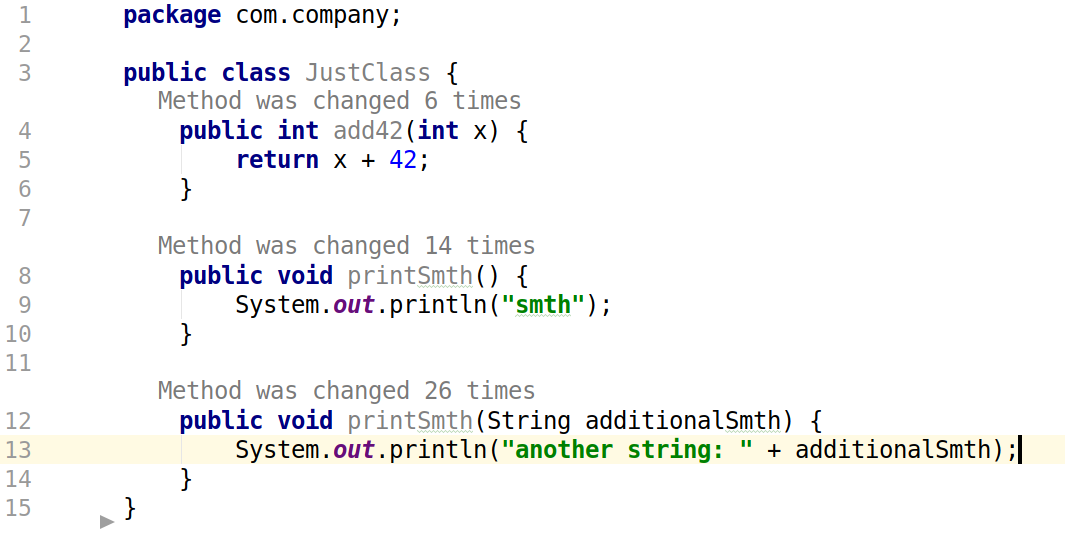
\includegraphics[width=\textwidth]{visual.png}
        \caption{Представление информации об изменениях метода\label{visual}}
    \end{figure*}

% У заключения нет номера главы
\section*{Заключение}
В ходе данной работы в течение осеннего семестра были достигнуты следующие результаты:
\begin{itemize}
    \item Реализован прототип плагина, интегрирующийся с SDK IntelliJ Platform для анализа изменений в системе контроля версий и отображения полученных данных в редакторе кода
    \item Для обработки рефакторингов произведена интеграция с RefactoringMiner
    \item Полученное решение корректно работает для небольших репозиториев с тривиальными изменениями
\end{itemize}

В ходе дальнейшей работы планируется оптимизировать решение для корректной работы с большими репозиториями, улучшить визуальное представление данных, сделать плагин конфигурируемым и опубликовать результат в репозитории плагинов JetBrains.
\section*{Листинги}

\begin{lstlisting}[language=Java, style=basic, caption={Пример работы с API RefactoringMiner}, captionpos=b, label=rminer]
GitService gitService = new GitServiceImpl();
GitHistoryRefactoringMiner miner = new GitHistoryRefactoringMinerImpl();

Repository repo = gitService.cloneIfNotExists(
    "tmp/refactoring-toy-example",
    "https://github.com/danilofes/refactoring-toy-example.git");
miner.detectAtCommit(repo, 
"https://github.com/danilofes/refactoring-toy-example.git",
    "05c1e773878bbacae64112f70964f4f2f7944398", new RefactoringHandler() {
  @Override
  public void handle(RevCommit commitData, List<Refactoring> refactorings) {
    System.out.println("Refactorings at " + commitData.getId().getName());
    for (Refactoring ref : refactorings) {
      System.out.println(ref.toString());
    }
  }
});
\end{lstlisting}
\setmonofont[Mapping=tex-text]{CMU Typewriter Text}
\bibliographystyle{ugost2008ls}
\bibliography{diploma.bib}
\end{document}
